\section{Study 1: the paired effect of retaining assistant replies}
\label{sec:study1}

\subsection{Design}

We used the math subset of Lost in Conversation \citep{laban2025lost}: 103
GSM8K-derived problems \citep{cobbe2021training}, each split into information
shards revealed one per turn. Before any model call, an input audit excluded 17
tasks that duplicated our earlier inputs or appeared to change meaning when
sharded, and a hash-based draw that used no model output selected \nTasks{}
tasks with 4--9 shards (median 6). GPT-4o-mini \citep{openai2024gpt4o}, Llama-4
Scout and Mistral-7B \citep{jiang2023mistral} answered every turn in both the
dialogue-history and fresh-prefix arms. Each reply had to end with
\texttt{FINAL\_ANSWER: <number>} or \texttt{STATUS: NEED\_MORE\_INFORMATION}.
Each cell received $K=\Krep{}$ samples and $L=\Lpar{}$ rewordings at
temperature \Ktemp{}; only the primary reply entered later history. All
\nRecords{} calls succeeded without truncation; six empty Mistral-7B primaries
were kept as invalid.

The primary endpoint was paired final-turn success, tested by exact McNemar
tests \citep{mcnemar1947note} with task-bootstrap 95\% intervals
(\nPermutations{} resamples; \citealp{efron1979bootstrap}) and Holm correction
across models \citep{holm1979simple}. Before the last shard most tasks have no
determined answer, so CQ, RS and ES cannot be observed; the pre-final warning
candidates were CS, LS and SS. Each was tested by a task-clustered partial
correlation with final failure, adjusted for model, turn, revealed information
and log context length, with Holm correction across the three metrics. CRL
(defined in Section~\ref{sec:framework}) measures delay in becoming ready to
answer, not accuracy; it targeted a positive final readiness gap, in which the
fresh prefix answers while the history arm is still waiting for information.

\subsection{Results}

\paragraph{Retaining assistant replies lowers final success (confirmatory)}
Final success fell from \freshGpt{} to \dialGpt{} for GPT-4o-mini (difference
\diffGpt{}, 95\% CI \ciGpt{}, Holm $p=\pHolmGpt$) and from \freshMistral{} to
\dialMistral{} for Mistral-7B (\diffMistral{}, CI \ciMistral{}, Holm
$p=\pHolmMistral$). Llama-4 Scout moved in the same direction (\diffLlama{}, CI
\ciLlama{}, Holm $p=\pHolmLlama$) without significance
(Table~\ref{tab:s1primary}, Figure~\ref{fig:s1}). Across models, only the fresh
prefix succeeded in \nFreshOnly{} model--task pairs and only the history arm in
\nDialOnly{}. The GPT-4o-mini and Mistral-7B effects remained when tasks with
format-invalid final replies were excluded (supplementary
Table~S1). For Mistral-7B the harm took a visible form: with
its own replies in context it tended to stay in the ``need more information''
state at the last turn, whereas without them it answered.

\begin{table}[!htbp]
\centering
\caption{Study 1 paired final-turn success over \nTasks{} tasks per model.
F/D: tasks in which only the fresh prefix, or only the dialogue history,
succeeded; $p$: exact McNemar test.}
\label{tab:s1primary}
\small
\resizebox{\linewidth}{!}{%
\begin{tabular}{lcccccc}
\toprule
Model & Dialogue history & Fresh prefix & Diff.\ [95\% CI] & F/D & $p$ & $p_{\text{Holm}}$\\
\midrule
\inputtable{generated/table_primary.tex}
\bottomrule
\end{tabular}
}
\end{table}

\begin{figure}[!htbp]
\centering
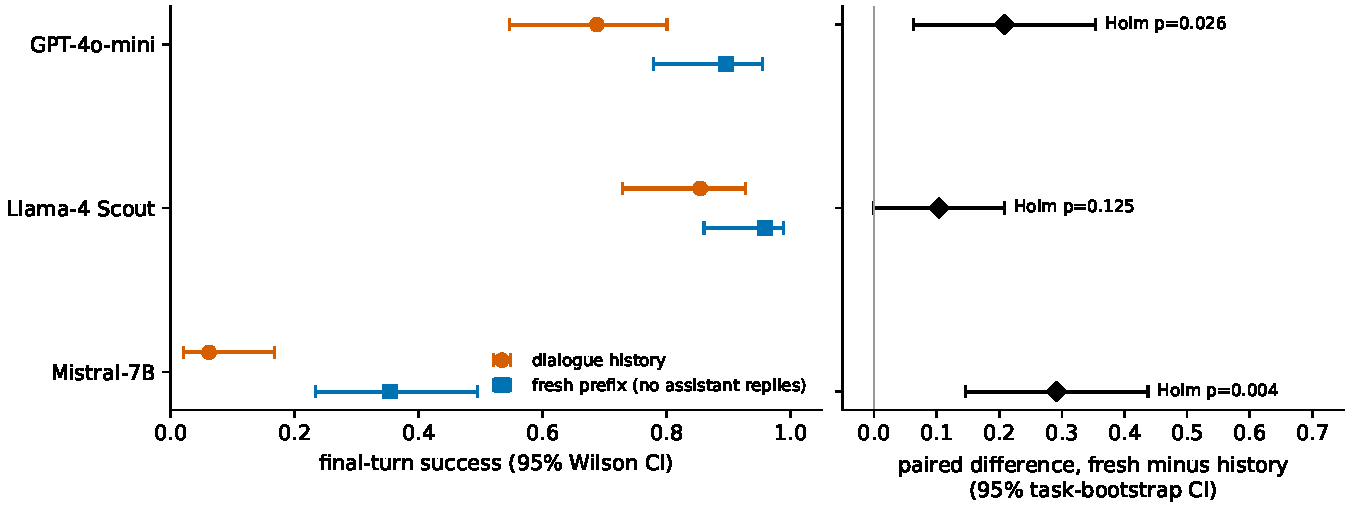
\includegraphics[width=\linewidth]{study1_paired.pdf}
\caption{Study 1 primary endpoint ($n=\nTasks{}$ paired tasks per model).
Left: final-turn success with 95\% Wilson intervals \citep{wilson1927probable}.
Right: paired difference, fresh prefix minus dialogue history, with 95\%
task-bootstrap intervals and Holm-adjusted McNemar $p$-values.}
\label{fig:s1}
\end{figure}

\paragraph{The measurable quality metrics do not warn (confirmatory)}
CS, LS and SS showed no statistically detectable association with final
failure beyond turn, revealed information and context length: all partial
correlations were close to zero and every Holm-adjusted $p$-value was 1.0
(Table~\ref{tab:s1rqeval}). This does not mean that they carry no information;
CS was measurable on only 29 source tasks, so small associations cannot be
excluded.

\begin{table}[!htbp]
\centering
\caption{Study 1 pre-final metrics as predictors of final failure under
dialogue history. A unit is one (task, model) pair (up to $3\times\nTasks{}$);
turns are the pre-final turns of those units pooled together, the level at
which the metric is observed; tasks are the distinct source tasks contributing
at least one turn, the level at which the permutation test clusters
observations. $r_{\text{partial}}$: task-clustered partial correlation; $p$:
one-sided task-clustered permutation test.}
\label{tab:s1rqeval}
\small
\begin{tabular}{lcccccc}
\toprule
Metric & Turns & Units & Tasks & $r_{\text{partial}}$ & $p$ & $p_{\text{Holm}}$\\
\midrule
\inputtable{generated/table_rqeval.tex}
\bottomrule
\end{tabular}
\end{table}

\paragraph{The paired readiness measure reduces to persistence}
CRL discriminated its target modestly (pooled model-stratified AUROC
\crlAuroc{}, permutation $p=\crlP$, CI \crlCi{}; supplementary
Table~S2). Post hoc, the last pre-final readiness gap alone did
better (AUROC \crlLastGapAuroc{}, $p=\crlLastGapP$), and within its strata CRL
added nothing (AUROC \crlCondAuroc{}, $p=\crlCondP$). Against accuracy loss, a
post-hoc target, the association was borderline (AUROC \robAllAuroc{},
$p=\robAllP$) and came from Mistral-7B alone. Even a paired, counterfactual
measure thus recorded the failure once the history arm had fallen behind
rather than anticipating it.
